\documentclass{article}
\usepackage{iclr2026_conference,times}
\input{math_commands.tex}
\usepackage{amsmath}
\usepackage{booktabs}
\usepackage{graphicx}
\usepackage{hyperref}
\usepackage{url}
\usepackage{array}
\usepackage{float}
\hypersetup{hidelinks,hypertexnames=false}
\renewcommand{\ttdefault}{cmtt}
\newcolumntype{L}[1]{>{\raggedright\arraybackslash}p{#1}}

\title{Potential-Guided Planning in Magic Tower:\\
A Deterministic Long-Horizon\\
Resource-Allocation Benchmark}

\author{
Bingsong Tong (2025310812), Zhizhou Qu (2025310268), Rui Chen (2025211105)\\
Deep Reinforcement Learning Course Project 2026
}

\iclrfinalcopy

\begin{document}
\raggedbottom
\maketitle
\lhead{Deep Reinforcement Learning Course Project 2026}

\begin{abstract}
Magic Tower is a deterministic single-agent role-playing puzzle in which the
agent must manage hit points (HP), attack (ATK), defense (DEF), keys, and money
across many irreversible interactions.  We study the first-ten-floor task, which
is fully observable and rule-defined, yet naive reinforcement learning rarely
receives a useful terminal signal.  The deterministic combat formula creates
sharp resource thresholds: a locally legal interaction may preserve immediate
feasibility while eliminating a much later solution path.  We organize the study
around three complementary approaches.  First, agent-assisted reference-route
construction produces high-quality trajectories for auditing simulator semantics
and revealing feasible resource schedules.  Second, an AlphaGo Zero-style
learning-and-planning pipeline combines a graph policy/value model,
single-agent PUCT-MCTS, and potential-based reward shaping learned from
reference trajectories.  The reference-aided policy/value variant reaches the
terminal condition from the fixed initial state with final HP \(315\), while the
no-demonstration variant remains incomplete.  Third, a multi-agent reference
planner decomposes legal candidate evaluation into stage, resource, combat, and
terminal-objective modules, obtains a validated trajectory with final HP
\(436\), and provides a prototype for future Magic Tower agent benchmarks with
symbolic, textual, and video observations.
\end{abstract}

\section{Introduction}
Magic Tower is a grid-based role-playing puzzle in which the agent ascends a
multi-floor tower by navigating corridors, collecting resources, opening doors,
triggering events, and fighting enemies.  Each floor is a discrete map whose
cells contain walls, stairs, consumable items, key-locked doors, enemies, or
non-player events.  The agent's state is summarized by its location and a small
set of persistent resources: HP, ATK, DEF, money, and colored keys.  A
single interaction may consume a map object, change the reachable region of the
tower, or permanently modify the agent's combat statistics.  Progress is
therefore not determined by local navigation alone, but by the order in which
the agent converts limited resources into future accessibility.

\begin{figure}[t]
  \centering
  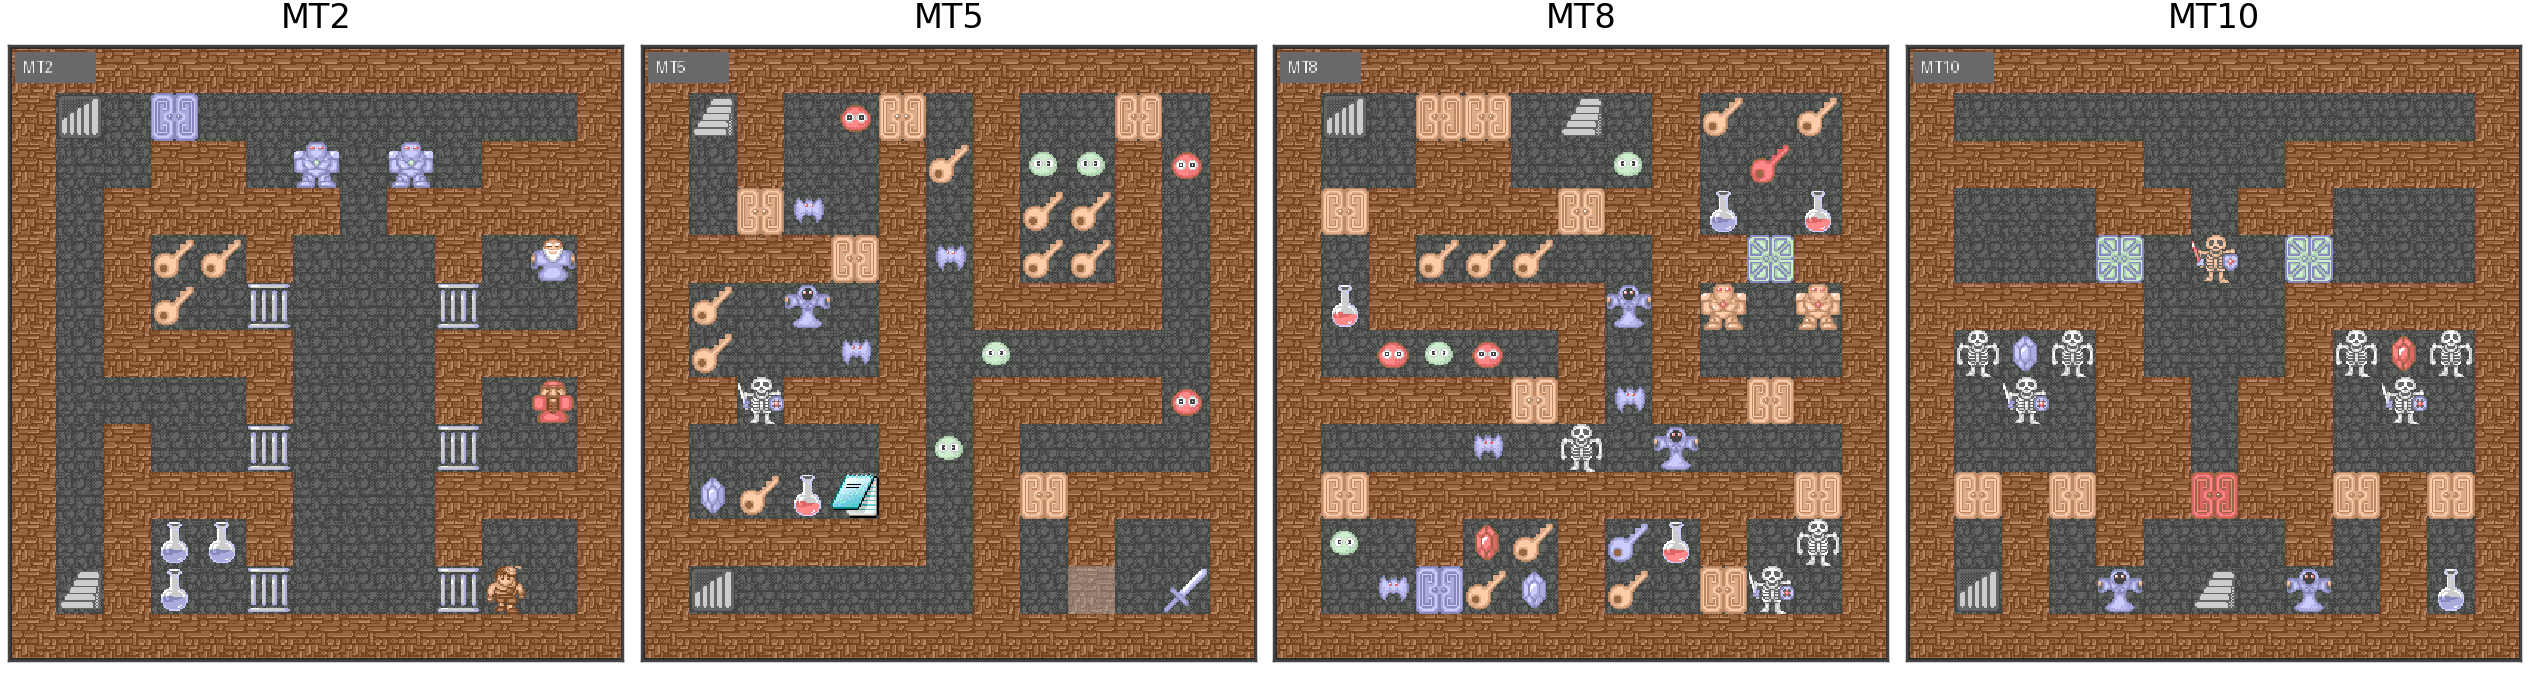
\includegraphics[width=0.95\linewidth]{figures/mota_floor_snapshots.png}
  \caption{Representative floors from the first-ten-floor Magic Tower instance.
  Each panel is a tile-rendered floor map: traversable corridors connect stairs,
  resource pickups, doors, enemies, and event triggers.  The figure illustrates
  why the task is a multi-floor resource-interaction problem rather than a
  purely local navigation problem.}
  \label{fig:floors}
\end{figure}

The game is fully observable and deterministic, but this does not make it
trivial for reinforcement learning.  Combat damage is computed by a fixed
formula from the agent and enemy statistics, so one additional point of ATK
or DEF can abruptly change the cost of multiple future encounters.  Doors
and consumable items introduce irreversible resource allocation: opening a
locally useful door may spend the key needed to access a later damage-reducing
item, while taking an HP potion too early may remove the buffer needed for a
more efficient future route.  As a result, Magic Tower is naturally modeled as a
deterministic long-horizon planning problem over a dynamically changing
resource-interaction graph.

We study a first-ten-floor instance in which success requires reaching the
terminal encounter with positive HP under deterministic validation.  The task
contains the core dependencies of the full game: early equipment acquisition,
key circulation, threshold-sensitive stat growth, and a terminal combat check.
This paper develops three complementary solution paths.  First, agent-assisted
reference-route construction is used to obtain high-quality trajectories and to
validate simulator semantics; an earlier human-audited reference route with
final HP \(403\) is retained for potential learning and simulator audits.
Second, we build an AlphaGo Zero-style learning-and-planning system that
combines graph policy/value learning, single-agent PUCT-MCTS, and
potential-based reward shaping.  The reference-aided policy/value variant solves
the first-ten-floor instance from the fixed initial state, reaching final HP
\(315\), whereas the no-demonstration variant still reaches only intermediate
milestones.  Third, a multi-agent beam-search planner constructs a strong
reference trajectory with final HP \(436\) by decomposing candidate evaluation
into stage, resource, combat, and terminal-objective modules.  Beyond improving
reference-route construction, this third line anticipates a benchmark setting in
which language or multimodal agents must coordinate specialized reasoning roles
over the same simulator-verified action interface.

\section{Related Work}
\paragraph{Search-guided reinforcement learning.}
AlphaGo Zero and AlphaZero demonstrated that policy/value networks can be
improved through Monte Carlo tree search without relying on handcrafted
evaluation functions \citep{silver2017mastering,silver2018general}.  These
systems train a network \(f_\theta(s)=(p_\theta(\cdot\mid s),v_\theta(s))\),
use MCTS to convert the raw policy prior into an improved visit-count policy,
and then regress the network back toward the search policy and realized return.
MCTS itself can be viewed as a repeated selection, expansion, evaluation, and
backup procedure whose action rule balances exploitation and uncertainty
\citep{kocsis2006bandit,browne2012survey}.  In AlphaZero-style PUCT, this
balance is further biased by a learned prior over legal actions.  These
systems, however, are designed for two-player board games with frequent
terminal supervision and alternating max/min structure.  Magic Tower is a
single-agent deterministic MDP: every decision layer is a maximization layer,
MCTS backups accumulate discounted task return without a sign flip, and random
interaction rarely reaches a successful terminal state.  MuZero further showed
that planning can be performed with a learned dynamics model
\citep{schrittwieser2020muzero}; in this project the transition model is known,
so the central question is not model learning but how to combine symbolic
simulation, policy/value priors, and long-horizon search.

\paragraph{Hard exploration and archive methods.}
Magic Tower belongs to the hard-exploration regime because most early action
sequences either exhaust resources or enter irreversible dead states before any
useful terminal reward is observed.  Go-Explore addresses this failure mode by
remembering promising intermediate states, returning to them, and exploring
outward from those stepping stones \citep{ecoffet2019goexplore}.  This idea is
well aligned with Magic Tower: a state after obtaining a key item, preserving a
key buffer, or satisfying a combat threshold is often more valuable than a
locally high-scoring route prefix.  The archive-MCTS component follows this
perspective by treating stage states as reusable search anchors rather than
restarting all exploration from the initial state.  Because the simulator is
deterministic, returning to an archived state can be implemented by storing the
state object or by replaying its route prefix; the later robustification idea in
Go-Explore is analogous to training a policy/value model from successful archive
trajectories, but is kept separate from pure exploration in this report.

\paragraph{Reward shaping and demonstrations.}
Sparse terminal rewards make direct reinforcement learning inefficient in
Magic Tower.  Potential-based reward shaping provides a principled way to add
dense feedback while preserving the optimal policy under suitable conditions
\citep{ng1999policy}.  Inverse reinforcement learning and maximum-entropy
trajectory modeling offer broader tools for inferring reward structure from
demonstrations \citep{ziebart2008maxent}.  Our use of successful trajectories
is narrower: reference routes define an ordered sequence of states from which a
stage-conditioned potential is estimated.  This potential supplies dense
search rewards, while final evaluation remains tied to deterministic task
success.  The important distinction is that the potential term
\(\gamma\Phi_\phi(s',g')-\Phi_\phi(s,g)\) changes intermediate learning signals
through a telescoping difference, whereas the terminal task criterion remains
unchanged.

\paragraph{Puzzle, roguelike, and reasoning benchmarks.}
Sokoban-style environments emphasize irreversible spatial constraints and
generalization across levels \citep{justesen2018sokoban}, while NetHack and
MiniHack emphasize symbolic observations, complex entity interactions, and
long-horizon decision making \citep{kuttler2020nle}.  Magic Tower sits between
these families: it is fully observable and deterministic like many puzzle
domains, yet its difficulty is dominated by numerical resource thresholds and
multi-floor dependency structure.  ARC-AGI is also relevant because it frames
intelligence as abstract rule inference and test-time adaptation
\citep{chollet2019measure,chollet2024arcprize,chollet2025arcagi2}.  The
interactive ARC-AGI-3 setting extends this line toward agents that infer goals
and dynamics through action \citep{arcprize2026arcagi3,rodionov2026executable}.
Magic Tower offers a complementary benchmark: it has explicit transition
dynamics, textual and video-renderable trajectories, and a large community
corpus of demonstrations and play episodes.

\section{Problem Modeling and Search Interface}
\subsection{Deterministic MDP}
We model the task as a finite-horizon deterministic single-agent MDP
\[
  \mathcal M=
  (\mathcal S,\mathcal A_{\mathrm{valid}},f,r_{\mathrm{task}},
  \gamma,\rho_0,\mathcal G,\mathcal F,H).
\]
All experiments use a fixed start state, so \(\rho_0\) is a point mass.  A state
\(s\in\mathcal S\) contains the complete map state of Floors 1--10, the
agent floor and coordinate, hero resources, key counts, consumed objects,
triggered events, and Boolean event variables.  We write
\(\mathrm{HP}(s)\), \(\mathrm{ATK}(s)\), \(\mathrm{DEF}(s)\), and
\(\mathrm{Money}(s)\) for the four numeric hero resources.  The valid
action set is the set of executable abstract actions:
\[
  a_t \in \mathcal A_{\mathrm{valid}}(s_t).
\]
Each action chooses an interaction node, not an individual arrow key.  The
simulator expands it into a shortest path to a reachable item, stair, event,
merchant, openable door, or killable enemy.  The transition is deterministic:
\[
  s_{t+1}=f(s_t,a_t).
\]
Let \(b_{\mathrm{term}}(s)\in\{0,1\}\) denote the terminal event variable set by
the simulator after the Floor-10 terminal adversary is defeated.  Terminal
success is the state set
\[
  \mathcal G=\{s\in\mathcal S:b_{\mathrm{term}}(s)=1
  \land \mathrm{HP}(s)>0\}.
\]
Failures include death, invalid transitions, timeouts, and dead states with no
useful executable actions; by construction \(\mathcal G\cap\mathcal F=\emptyset\).
The sparse task reward is
\[
  r_{\mathrm{task}}(s,a,s') =
  R_G\mathbf 1[s'\in\mathcal G]
  -R_F\mathbf 1[s'\in\mathcal F]
  -\kappa,
\]
where \(\kappa\) is a small abstract-step cost.  For terminal states we set
\(V^*(s)=0\).  For non-terminal states, the optimal value satisfies the
single-player Bellman equation
\[
  V^*(s)=
  \max_{a\in\mathcal A_{\mathrm{valid}}(s)}
  \left[r_{\mathrm{task}}(s,a,f(s,a))+\gamma V^*(f(s,a))\right].
\]
This yields an AlphaGo Zero-style search interface, but the target is a
deterministic single-agent return rather than an adversarial game outcome.  A
PUCT-MCTS rollout backs up
\[
  G_k = r_k+\gamma G_{k+1}
      = \sum_{i=k}^{L-1}\gamma^{i-k}r_i+\gamma^{L-k}\hat V(s_L).
\]
The search policy at the root is obtained from visit counts,
\[
  \pi_{\mathrm{MCTS}}(a\mid s)
  =
  \frac{N(s,a)^{1/\tau}}
  {\sum_{b\in\mathcal A_{\mathrm{valid}}(s)} N(s,b)^{1/\tau}},
\]
and an AlphaZero-style single-agent learner would train on triples
\((s_t,\pi_{\mathrm{MCTS}}(\cdot\mid s_t),G_t)\), replacing the two-player
win/loss label with cumulative task return.

Combat is the main discontinuity.  For an ordinary enemy \(e\), let
\((H_e,A_e,D_e)\) be enemy HP, ATK, and DEF, and let
\((A_h(s),D_h(s))\) be hero ATK and DEF.  If \(A_h(s)\le D_e\), the enemy is
not killable.  Otherwise, the number of hero attacks is
\[
  T(s,e)=
  \left\lceil \frac{H_e}{A_h(s)-D_e} \right\rceil,
\]
and the ordinary combat loss implemented by the simulator is
\[
  C(s,e) =
  (T(s,e)-1)\max(0,A_e-D_h(s)).
\]
The factor \(T-1\) reflects that the enemy does not counterattack after the
final hero strike.  The simulator adds the configured first-strike, fixed-damage,
counterattack, and armor-breaking terms for enemies that carry special effects.
Thus a single red or blue gem can reduce future damage by hundreds of HP, while
the same gem may have no effect away from a threshold.  This makes dense reward
design unusually sensitive.

\subsection{Simulator and Macro-Action Interface}
\label{subsec:macro_action}
The simulator is implemented in Python and uses the extracted HTML5 data as the
truth source.  It implements deterministic combat, resource collection, doors,
stairs, merchants, and event transitions required by the first-ten-floor
instance.  The visualizer is kept as an independent validation interface; search
and learning interact only with the simulator state.

Primitive arrow-key control is unnecessarily long-horizon for planning.
Instead, the agent chooses an interaction node.  For a state \(s\) on floor
\(f\), let \(G_f=(V_f,E_f)\) be the precomputed static adjacency graph of
walkable grid cells, and let \(B_f(s)\subset V_f\) be the dynamic blocker set
containing currently closed doors, undefeated enemies, blocking events, and
non-pass-through NPC cells.  Reachability is computed on the induced graph
\[
  G_f(s)=G_f[V_f\setminus B_f(s)].
\]
A single BFS from the hero position gives the reachable set \(R_f(s)\), distances
\(\mathrm{dist}_s(v)\), and a parent pointer
\[
  \mathrm{par}_s(v)=(u,\delta),\qquad u\in R_f(s),\ \delta\in\{\uparrow,\downarrow,\leftarrow,\rightarrow\}.
\]
The macro-action set is then generated in two passes.  First, every reachable
interaction node is executable immediately.  Second, each blocker adjacent to
\(R_f(s)\) becomes a candidate door, enemy, or event action, and a local legality
predicate checks keys, battle survivability, money, and event flags:
\[
  \mathcal A_{\mathrm{valid}}(s)
  =
  \{a_i:i\in I_f,\ i\in R_f(s)\}
  \cup
  \{a_j:j\in \partial R_f(s),\ L(s,j)=1\}.
\]
This abstraction keeps ordinary movement inside the transition function while
preserving all resource-changing decisions and floor-transfer choices as
abstract actions.

The expensive part is not BFS itself, since each floor has only a small fixed
grid; the cost comes from repeating it inside thousands of tree expansions and
allocating full paths for targets that are never selected.  We therefore use a
fast reachability layer: static adjacency lists and interaction-node tables are
precomputed once, \(B_f(s)\) is encoded as a compact bitset, BFS results are
cached by \((f,\mathrm{pos}(s),B_f(s))\), and paths are reconstructed from
\(\mathrm{par}_s\) only for the chosen action.  Scalar variables such as HP,
ATK, DEF, money, and keys are excluded from the BFS cache key; they affect only
the local legality predicate \(L(s,j)\), not geometric passability.  This
separation reduces CPU time in MCTS by turning most action enumeration calls into
bitset lookup, cached reachability, and cheap local legality checks.

\subsection{Evaluation Setting and Reference Trajectories}
For validation and later comparison, we construct high-quality reference
trajectories with external planning assistance and strict simulator replay.  The
purpose is to expose feasible resource schedules, validate the simulator, and
establish reference behavior for subsequent reward and planning experiments.
These trajectories verify deterministic transition semantics, event logic,
and visualization consistency.  The fixed start
state is Floor 2 at coordinate \((3,7)\), with
\(\mathrm{HP}=400\), \(\mathrm{ATK}=10\), \(\mathrm{DEF}=10\),
\(\mathrm{Money}=4\), and zero colored keys.  The reference trajectory reaches the
Floor-10 terminal condition with
\[
  \mathrm{HP}_T=403,\quad
  \mathrm{ATK}_T=27,\quad
  \mathrm{DEF}_T=27,\quad
  \mathrm{Money}_T=262.
\]
The trajectory is retained as a validation artifact, not as evidence that the
pure RL system has solved the task.

\section{Methodology}
\subsection{Reference-Derived Potential Learning}
\label{subsec:potential}
The reference trajectory is too narrow to define the full optimal policy.
We therefore use it as an ordered sequence of states for estimating a potential
function
\(\Phi_\phi(s,g)\), following the policy-invariance motivation of
potential-based reward shaping \citep{ng1999policy}.  For a successful trajectory
\(\tau=(s_0,a_0,\ldots,s_T)\), we create progress and ranking labels:
\[
  y_t = t/T,\qquad s_j \succ s_i \quad \text{if } j>i.
\]
The potential loss combines regression, pairwise ranking, and dead-end
separation:
\[
  \begin{aligned}
  \mathcal L_\Phi(\phi)
  ={}& \sum_t(\Phi_\phi(s_t,g_t)-y_t)^2 \\
  &-\alpha\sum_{j>i}
  \log\sigma(\Phi_\phi(s_j,g_j)-\Phi_\phi(s_i,g_i))\\
  &-\beta\sum_{(s^+,s^-)}
  \log\sigma(\Phi_\phi(s^+,g^+)-\Phi_\phi(s^-,g^-)).
  \end{aligned}
\]
Let \(g(s)\) denote the deterministic stage label associated with state \(s\).
The search reward is then potential-based.  With \(g=g(s)\) and \(g'=g(s')\)
denoting the stage labels before and after the transition,
\[
  r_{\mathrm{search}}(s,g,a,s',g') =
  r_{\mathrm{task}}(s,a,s')
  +\lambda\left(\gamma\Phi_\phi(s',g')-\Phi_\phi(s,g)\right).
\]
Along a finite trajectory, the discounted sum of the shaping term telescopes:
\[
  \sum_{t=0}^{T-1}\gamma^t
  \left(\gamma\Phi_\phi(s_{t+1},g_{t+1})-\Phi_\phi(s_t,g_t)\right)
  =
  -\Phi_\phi(s_0,g_0)+\gamma^T\Phi_\phi(s_T,g_T).
\]
Here \(g_t=g(s_t)\), so the stage-conditioned potential is equivalently a
potential over an augmented Markov state.  Strict policy invariance follows in
the standard absorbing-state formulation, or when terminal-state potentials are
fixed so that the final term does not distinguish successful terminal states.
In this project the shaped reward is therefore treated as a search and learning
signal rather than as the evaluation objective.
Thus the potential can bias local learning and search toward states that look
closer to success, while the original terminal objective remains the quantity
used for evaluation.
This keeps task evaluation separate from shaping.  Final success is always
measured by deterministic validation and the terminal predicate
\(b_{\mathrm{term}}\), not by shaped reward.

We use a linear potential over audited semantic factors rather than a free-form
neural reward model.  Let
\(c_k(s;g)\) denote the \(k\)-th stage-conditioned component for stage \(g\),
including agent resources, key pressure, reachable resources, blocked resource
pressure, monster damage, marginal damage decrease under ATK+1 or DEF+1,
equipment progress, Floor-10 resource progress, and terminal-feasibility
margin.  The learned
potential is
\[
  \Phi_\phi(s,g)=
  \sum_k w_{g,k}c_k(s;g)+\sum_k w^{\mathrm{global}}_k c_k(s;g).
\]
For later notation, let
\(\bar w_{g,k}=w_{g,k}+w^{\mathrm{global}}_k\) denote the effective component
weight.

The reference trajectory is used to estimate only the weights \(w_{g,k}\), not the
feature definitions.  Each component \(c_k\) is computed from the simulator and
resource graph.  We group the components as
\[
  c(s;g)=
  \left[
  c^{\mathrm{hero}},
  c^{\mathrm{key}},
  c^{\mathrm{reach}},
  c^{\mathrm{combat}},
  c^{\mathrm{threshold}},
  c^{\mathrm{stage}},
  c^{\mathrm{terminal}}
  \right].
\]
The reference trajectory provides stage-specific constraints on the relative
weights of these groups at different
stages.  The hero block contains HP, ATK, DEF, money, and key counts.  The key
and reachability blocks measure current key pressure, executable resources, and
resources blocked by doors or enemies.  The combat block contains deterministic
damage to killable enemies and the terminal adversary.  The threshold block
contains marginal damage drops under one additional ATK or DEF:
\[
  \Delta_a(s,e)=C(s,e)-C(s^{a+1},e),\qquad
  \Delta_d(s,e)=C(s,e)-C(s^{d+1},e),
\]
where \(s^{a+1}\) and \(s^{d+1}\) denote counterfactual states with one extra
ATK or DEF.  The stage block records milestone progress such as equipment,
stat resources, key items, and terminal-gate readiness, while the terminal block
contains the final HP margin and the terminal event variable.

Training examples compare one-step potential changes among legal abstract
actions.  Define
\[
  \Delta_\phi(s,a;g)
  =
  \gamma\Phi_\phi(f(s,a),g(f(s,a)))-\Phi_\phi(s,g),
\]
where the next-stage label is evaluated after applying the transition.  At trajectory step
\(t\), the simulator enumerates
\(\mathcal A_{\mathrm{valid}}(s_t)\).  The reference transition
\((s_t,a^E_t,f(s_t,a^E_t))\) provides
a positive ranking candidate for the one-step potential difference:
\[
  \Delta_k^E =
  \gamma c_k(f(s_t,a^E_t);g(f(s_t,a^E_t)))-c_k(s_t;g_t),
\]
and each valid alternative \(a^-\) provides
\[
  \Delta_k^- =
  \gamma c_k(f(s_t,a^-);g(f(s_t,a^-)))-c_k(s_t;g_t).
\]
The ranker optimizes
\[
  \mathcal L_{\mathrm{rank}}
  =
  \sum_{t,a^-}
  \mathrm{softplus}\left(
  -\sum_k \bar w_{g_t,k}(\Delta_k^E-\Delta_k^-)
  \right)
  +\eta\|w\|_2^2.
\]
Here \(\bar w_{g_t,k}\) includes both the stage-specific and global
contributions.
Equivalently, the learned potential is trained so that
\[
  \Delta_\phi(s_t,a^E_t;g_t)
  >
  \Delta_\phi(s_t,a;g_t),
  \qquad
  a\in\mathcal A_{\mathrm{valid}}(s_t)\setminus\{a^E_t\},
\]
whenever the reference action advances the successful reference route more than
the legal alternative.  Dead-end search states add negative pairs by requiring
states on successful prefixes to have larger potential than states that have no
useful continuation.  Thus the reference data affect the learned shaping term
through stage-specific factor weights, progress labels, and pairwise transition
preferences.  They do not alter the sparse terminal reward, the transition
function, the action mask, or the PUCT policy prior.
The output is therefore a stage-conditioned potential, not a policy prior.
The downstream AlphaZero-style and archive-MCTS experiments use the
reference trajectory only
through
\[
  r_{\Phi}(s,g,a,s',g')=\gamma\Phi_\phi(s',g')-\Phi_\phi(s,g),
\]
  which enters single-agent MCTS backups as an edge reward and value-return
target.  The potential-only experiment uses no reference prefix or reference
action prior during search.

\subsection{Multi-Agent Reference Planner}
The reference-construction line uses the same simulator and legal macro-action
interface, but decomposes candidate evaluation into specialized scoring modules.
At state \(s_t\), the simulator enumerates the legal candidate set
\(\mathcal A_{\mathrm{valid}}(s_t)\) and computes the deterministic successor
\(s^a=f(s_t,a)\) for each candidate.  All modules observe the same tuple
\[
  x(s_t,a)=
  \left(s_t,a,s^a,\mathcal A_{\mathrm{valid}}(s_t),m_t,\mathcal V_t\right),
\]
where \(m_t\) is a recent trace memory and \(\mathcal V_t\) is a visited-state
memory.  The modules score each candidate from complementary perspectives:
stage progress, key and item economy, combat thresholds, terminal-objective
readiness, and optional reference-route alignment.  If \(q_j(s,a)\) denotes the
score from module \(j\), the arbiter uses
\[
  S(s,a)=
  \sum_j \omega_j q_j(s,a)
  +\omega_{\mathrm{ref}}q_{\mathrm{ref}}(s,a)
  -\lambda_{\mathrm{loop}}\mathbf 1[\kappa(s^a)\in\mathcal V_t],
\]
where \(\kappa(s)\) is a compact state key used for loop suppression.  The
reference-alignment term is used only in this reference planner; it is not part
of the no-demonstration archive or pure PUCT experiments.

The arbiter performs beam search over simulator-verified transitions.  Given a
beam \(\mathcal B_t=\{(s_i,\tau_i,R_i)\}_{i=1}^K\), the next beam is
\[
  \mathcal B_{t+1}
  =
  \operatorname{TopK}_{(s_i,a)}
  \left\{
  \left(f(s_i,a),\tau_i\!\circ\!a,
  R_i+S(s_i,a)\right):
  a\in\mathcal A_{\mathrm{valid}}(s_i)
  \right\}.
\]
The planner therefore never edits the game state directly: every candidate
route is a sequence of legal simulator transitions.  Recent trace memory records
the latest stages, actions, and resource summaries, while visited-state memory
penalizes repeated floor-transition loops and semantically equivalent revisits.
This design provides a high-quality reference-route construction mechanism and
diagnostic traces for later potential learning, without changing the terminal
evaluation criterion.

\begin{figure}[t]
  \centering
  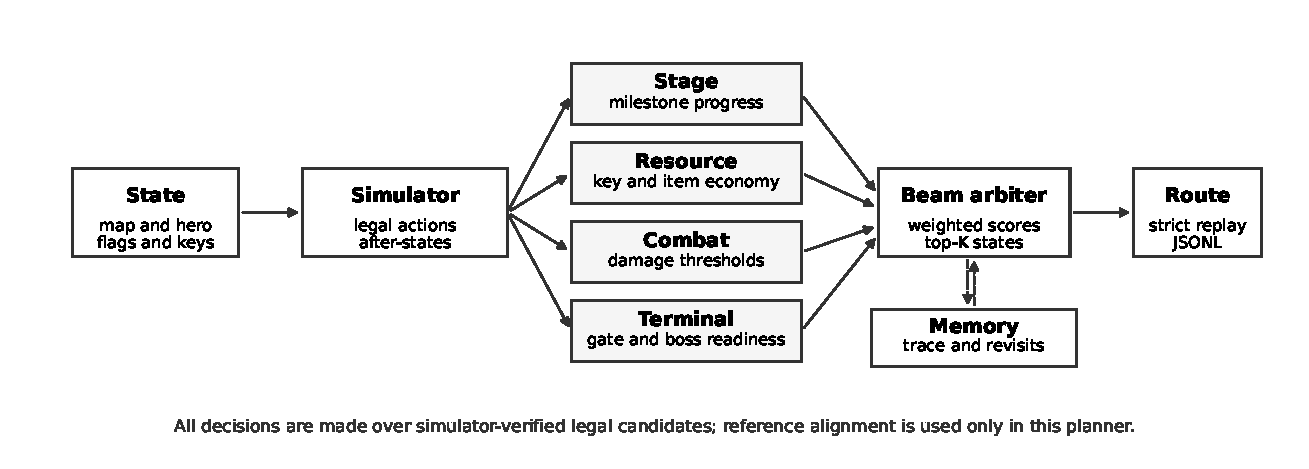
\includegraphics[width=0.96\linewidth]{figures/agentic_architecture.pdf}
  \caption{Multi-agent reference planner.  The simulator enumerates legal
  macro-actions and candidate after-states; specialized scoring modules evaluate
  the same candidate table; a beam-search arbiter combines scores, consults
  recent and visited-state memories, and writes a replayable route.}
  \label{fig:agentic-architecture}
\end{figure}

\subsection{Archive-Guided PUCT-MCTS}
The no-demonstration exploration line combines a global archive with local MCTS.  A cell
abstraction maps states to coarse stepping stones:
\[
  \chi(s)=
  (\mathrm{stage},\mathrm{floor},a_b,d_b,k_b,h_b,
   \mathrm{F10\_progress},\mathrm{terminal\_margin}_b).
\]
The archive stores top-\(K\) non-identical candidates per cell:
\[
  \mathcal B[\chi(s)] =
  \{(s_i,\tau_i,\mathrm{score}_i)\}_{i=1}^K.
\]
At each iteration, the algorithm first returns to a selected cell and then
explores from it.  The cell is sampled according to novelty, progress, and
visit penalty.  From the archived state \(s_c\), PUCT-MCTS selects a local
action:
\[
  a =
  \arg\max_{a\in\mathcal A_{\mathrm{valid}}(s)}
  \left[
  Q(s,a)+c_{\mathrm{puct}}P(s,a)
  \frac{\sqrt{\sum_{b\in\mathcal A_{\mathrm{valid}}(s)}N(s,b)}}{1+N(s,a)}
  \right].
\]
For the pure line \(P\) is uniform or learned from self-generated search traces,
not from reference routes.  In the potential-shaping line, the reference
trajectory influences only the
edge reward and leaf value through \(\Phi_\phi\).  The archive score is
lexicographic in success, stage progress, HP, keys, and path length, so a
high shaping score cannot replace task success.

\begin{figure}[t]
  \centering
  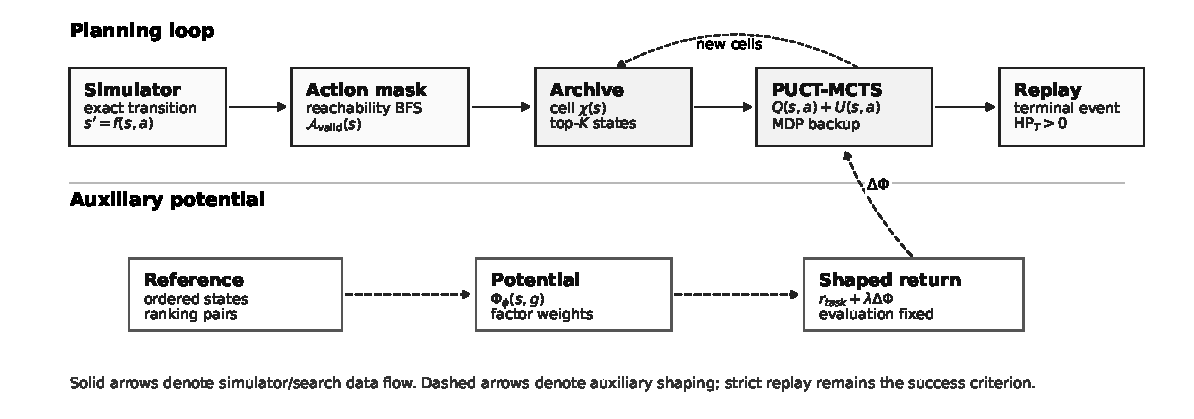
\includegraphics[width=\linewidth]{figures/system_diagram.pdf}
  \caption{System architecture.  The simulator provides deterministic abstract
  transitions and resource-graph states; archive search and PUCT operate on this
  symbolic interface, while visualization is used only for independent
  trajectory inspection.}
  \label{fig:system}
\end{figure}

\section{Empirical Results}
\paragraph{Evaluation criterion.}
All reported successes are verified by exact deterministic replay.  A trajectory
\(\tau=(s_0,a_0,\ldots,s_T)\) is counted as successful only if it reaches the
terminal event and retains positive hit points:
\[
  \mathrm{Eval}(\tau)=
  \mathbf 1[b_{\mathrm{term}}(s_T)=1 \land \mathrm{HP}(s_T)>0].
\]
Potential scores, shaped returns, supervised losses, and search scores are used
only as diagnostic quantities.  This separation is important because a shaped
reward can improve local search without certifying that the task objective has
been reached.  We therefore distinguish reference validation, potential
learning, reference-aided policy/value search, perturbation diagnostics, and
no-demonstration archive search.

\begin{figure}[t]
  \centering
  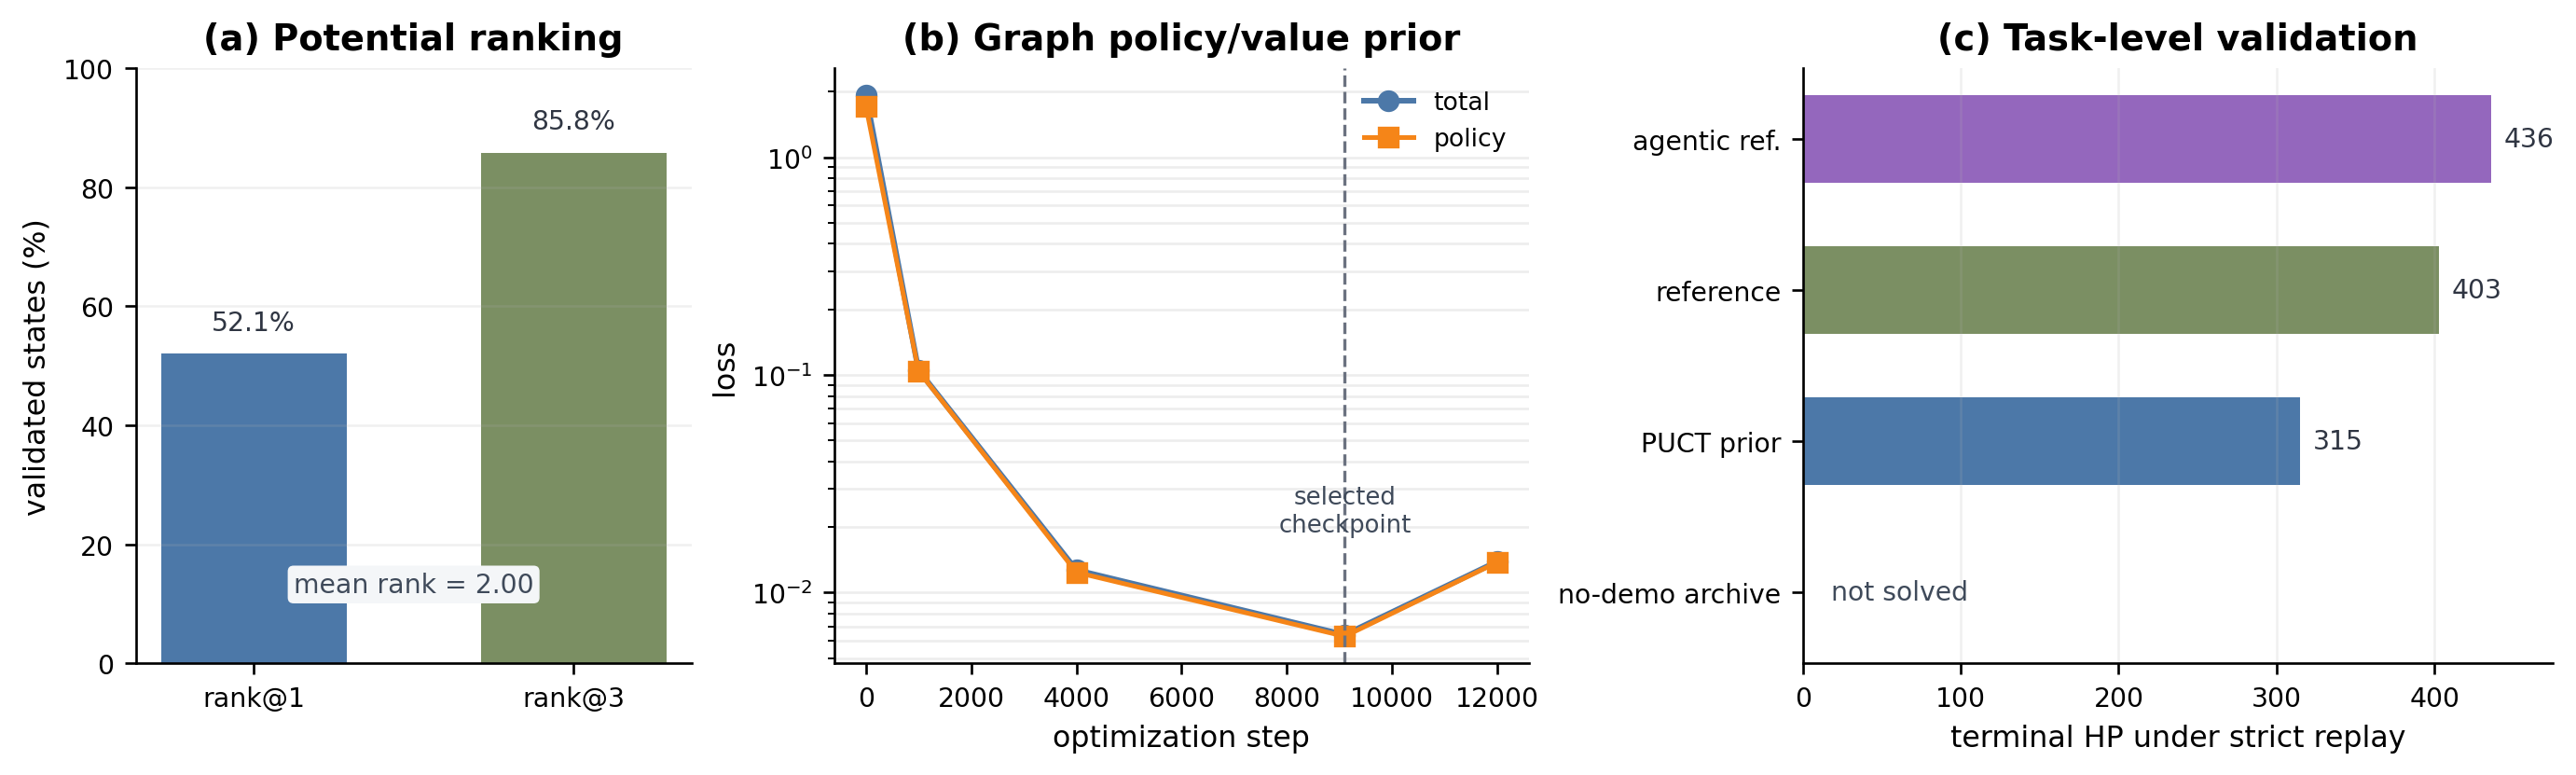
\includegraphics[width=0.98\linewidth]{figures/experiment_summary.png}
  \caption{Diagnostic summary of the three empirical signals used in this
  study.  The left panel evaluates whether the learned potential assigns higher
  progress to validated successors than to alternative legal successors.  The
  middle panel reports the supervised fit of the graph policy/value model used
  as a PUCT prior.  The right panel reports strict replay outcomes, which remain
  the only success criterion.  Thus, the figure separates shaping quality,
  model fitting, and task-level validation rather than treating shaped reward as
  a proxy for success.}
  \label{fig:experiment-summary}
\end{figure}

\paragraph{Potential learning.}
The potential model is trained from ordered states rather than from direct
action imitation.  For each validated transition we compare the reference
successor \(s^+\) with alternative legal successors \(s^-\), and optimize a
pairwise ranking objective
\[
  \mathcal L_\Phi(\phi)=
  -\sum_{(s^+,s^-)}
  \log \sigma\!\left(\Phi_\phi(s^+,g^+)-\Phi_\phi(s^-,g^-)\right).
\]
The resulting dataset contains \(317\) validated states and \(1578\) pairwise
comparisons.  The learned potential ranks the reference transition first in
\(52.1\%\) of states and within the top three in \(85.8\%\), with mean rank
\(2.00\).  These numbers measure shaping quality rather than policy
accuracy: \(\Phi_\phi\) only biases search through
\(\gamma\Phi_\phi(s',g')-\Phi_\phi(s,g)\), while the sparse terminal criterion
remains unchanged.

\paragraph{Graph policy/value model.}
The reference-aided comparison uses \(9\) unique successful trajectories
after exact action-sequence deduplication, yielding \(2576\) graph-state
supervision samples.  The model is a six-layer Transformer with
\(d_{\mathrm{model}}=512\), eight attention heads, dropout \(0.03\), batch size
\(512\), and AdamW learning rate \(8\cdot 10^{-5}\).  It maps a graph state and
stage token to a masked action prior and a scalar value estimate:
\[
  f_\theta(G_s,g)=
  \left(p_\theta(\cdot\mid s,g),v_\theta(s,g)\right),
\]
trained with
\[
  \mathcal L(\theta)=
  -\pi^\top\log p_\theta(\cdot\mid s,g)
  +0.35\,(G-v_\theta(s,g))^2
  +10^{-4}\|\theta\|_2^2.
\]
The best checkpoint occurs at step \(9100\), with total loss \(0.0064\) and
policy loss \(0.0063\).  The subsequent increase in policy loss is consistent
with the limited diversity of the successful-trajectory set.  We therefore use
the model as a search prior inside PUCT rather than treating it as an autonomous
policy.

\paragraph{Multi-agent reference planning.}
The multi-agent reference planner produces a legal trajectory of \(291\)
macro-actions.  Under strict replay, the terminal event is reached at the final
Floor-10 encounter with
\[
  \mathrm{HP}_T=436,\qquad
  \mathrm{ATK}_T=27,\qquad
  \mathrm{DEF}_T=27.
\]
The route passes the same deterministic replay validation as the other reported
routes.  Its milestone sequence is useful because it exposes the
long-horizon structure that local greedy search repeatedly misses: the route
obtains the sword at step \(19\), obtains the shield at step \(75\), collects
late Floor-10 stat resources before the terminal stage, obtains the red key at
step \(248\), opens the terminal red door at step \(281\), triggers the
Floor-10 mechanism at step \(282\), and reaches terminal success at step
\(290\).  The resource curves show that the route does not monotonically
maximize HP; instead, it accepts controlled HP losses to improve ATK and DEF,
then rebuilds the HP margin before the terminal sequence.

\begin{figure}[t]
  \centering
  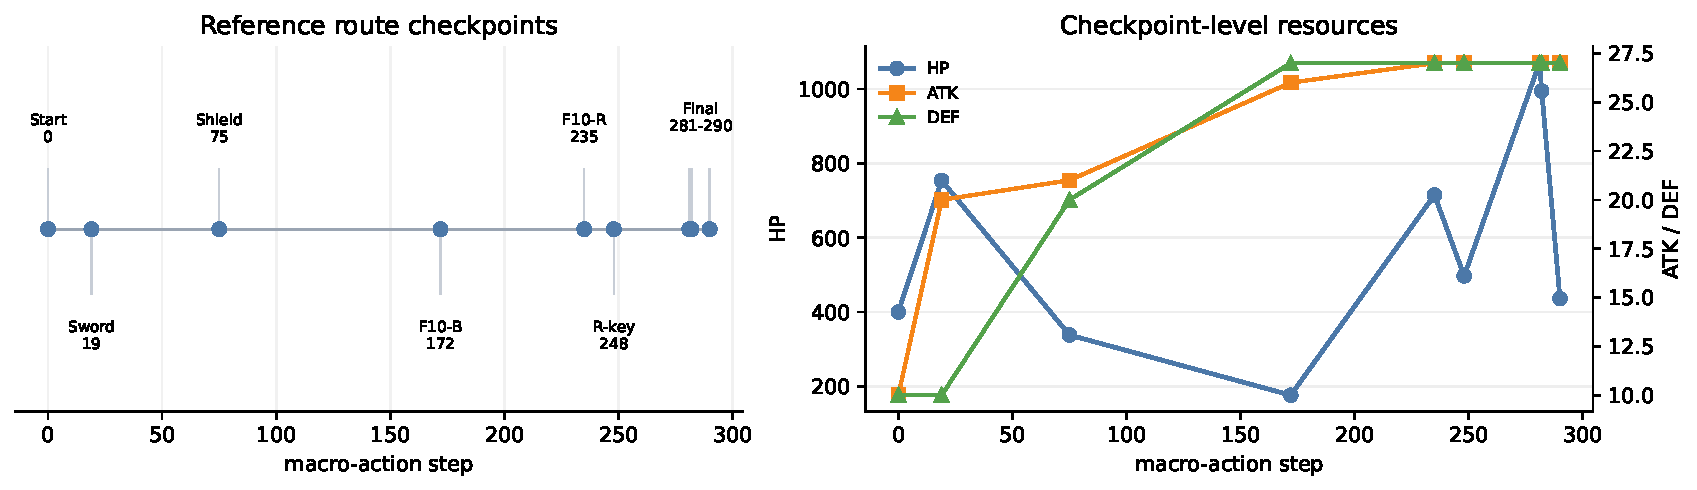
\includegraphics[width=0.98\linewidth]{figures/agentic_route_summary.pdf}
  \caption{Route structure of the multi-agent reference planner.  Left:
  checkpoint timing along the macro-action sequence.  Right: checkpoint-level
  HP, ATK, and DEF values, showing the trade-off between immediate hit-point
  loss and later combat-threshold improvement.}
  \label{fig:agentic-results}
\end{figure}

\begin{table}[t]
\centering
\small
\begin{tabular}{@{}L{0.22\linewidth}L{0.20\linewidth}L{0.18\linewidth}L{0.31\linewidth}@{}}
\toprule
Condition & Evidence source & Evaluation & Outcome\\
\midrule
Reference validation & Human-audited route & Strict replay & Terminal event reached with \(\mathrm{HP}_T=403\); used to validate simulator semantics and reward factors.\\
Multi-agent reference planner & Specialized scorers and beam arbiter & Strict replay & Terminal event reached in \(291\) macro-actions with \(\mathrm{HP}_T=436\), \(\mathrm{ATK}_T=27\), and \(\mathrm{DEF}_T=27\).\\
Potential shaping & Ordered states & Pairwise ranking & Rank@1 is \(52.1\%\), Rank@3 is \(85.8\%\), and mean rank is \(2.00\).\\
Policy/value search & Successful routes & PUCT & Closed-loop search reaches the terminal event from the fixed initial state with \(\mathrm{HP}_T=315\).\\
Layout perturbation & Modified resource layout & PUCT & The model does not reliably recover a relocated late-stage stat resource.\\
No-demonstration archive & Simulator-generated traces & Archive-MCTS & Several milestones are reached, but terminal success has not yet been obtained.\\
\bottomrule
\end{tabular}
\caption{Primary empirical outcomes.  Success is reported only under strict
deterministic replay; all other quantities are diagnostic signals used to
interpret shaping, search, and generalization behavior.}
\label{tab:result-summary}
\end{table}

\paragraph{Closed-loop validation.}
The policy/value model is useful only when coupled with search over the complete
legal abstract-action set.  Stage-restricted action filters can remove recovery
actions after small deviations and thereby obscure the value of the learned
prior.  With the full legal action set, PUCT solves the first-ten-floor task from
the fixed initial state, ending with \(\mathrm{HP}_T=315\),
\(\mathrm{ATK}_T=27\), and \(\mathrm{DEF}_T=27\).
Additional terminal-HP sweeps with the same architecture produced successful
trajectories, but did not improve upon this checkpoint.  The result supports a
narrow conclusion: the learned prior is an effective guide on the original
instance, but the experiment does not yet establish robust policy learning.

\paragraph{Generalization and exploration diagnostics.}
Two diagnostic tests expose the current limitations.  First, local item-swap
perturbations show that the model is sensitive to object relocation: when a
late stat resource is exchanged with a nearby key, closed-loop PUCT follows the
training-distribution route structure and does not reliably recover the moved
stat resource.  Second, PUCT can solve several suffix subproblems when
initialized from meaningful intermediate states, but independently generated
stage states do not compose reliably.  The dominant failure is continuation
awareness: a locally successful stage may consume the key or HP buffer required
by a later stage.

\begin{table}[t]
\centering
\small
\begin{tabular}{@{}L{0.28\linewidth}L{0.24\linewidth}L{0.40\linewidth}@{}}
\toprule
Diagnostic & Result & Interpretation\\
\midrule
Full-action PUCT & terminal success with \(\mathrm{HP}_T=315\) & Search benefits from learned priors when the legal mask preserves recovery actions.\\
Suffix planning & local suffixes solved & Intermediate-state reuse is necessary for composing long routes.\\
Stage composition & terminal event not reached & Stage values must encode future feasibility, not only immediate resource completion.\\
Resource relocation & late stat resource missed & The current model relies too strongly on layout-specific route structure.\\
No-demonstration archive & incomplete terminal progress & Exploration remains the central bottleneck without reference-derived signals.\\
\bottomrule
\end{tabular}
\caption{Diagnostic experiments.  The table separates what is already solved by
search-guided priors from the remaining weaknesses in stage composition,
object-relocation generalization, and no-demonstration exploration.}
\label{tab:diagnostics}
\end{table}

Finally, profiling shows that planning is simulator-bound rather than
neural-inference-bound.  The main costs are action enumeration, reachability
computation, state copying, and local legality checks.  This observation is
important for interpreting model scale: increasing the policy/value model size
is unlikely to improve search until the symbolic expansion layer uses compact
state encodings, transposition tables, reachability caches, lazy path recovery,
and batched leaf evaluation.

\section{Future Work: Magic Tower as an LLM Benchmark}
Magic Tower can be turned into a benchmark suite beyond this first-ten-floor
RL project.  The environment can expose three synchronized interfaces: symbolic
JSON state, natural-language state summaries, and video frames from the
visualizer.  An LLM agent can then be evaluated on action selection,
trajectory-level planning, rule discovery, and post-hoc explanation.  This is
analogous to ARC-AGI's emphasis on test-time reasoning, but Magic Tower adds an
explicit transition function and long interactive trajectories.

The multi-agent reference planner provides a concrete bridge to this benchmark
formulation.  Its modules already operate over a shared candidate-action table,
simulator-derived after-states, and explicit trace memory.  In a future
benchmark, these modules can be replaced by language or multimodal agents that
receive symbolic states, textual summaries, or video observations, while the
arbiter and strict simulator replay keep evaluation grounded in valid actions.
Thus the third approach studied here is not only a route-construction baseline;
it is also a minimal protocol for evaluating coordinated agent reasoning in
Magic Tower.

A major advantage of this domain is data scale.  The Magic Tower community has
produced thousands of user-created tower instances and a large number of
demonstrations, walkthroughs, and complete play episodes.  This corpus can
support multiple benchmark tracks: supervised trajectory modeling from
successful play, offline RL from mixed-quality episodes, reward learning from
ordered demonstrations, and held-out generalization across map layouts and tower
designs.  A robust benchmark must separate seen towers, unseen towers, rule
preserving layout perturbations, and observation modalities such as symbolic
state, text-only summaries, and video-only interaction.  This would make Magic
Tower a useful complement to ARC-style reasoning benchmarks: it preserves
symbolic rule structure while requiring long-horizon interactive resource
planning.

\section{Limitations}
This study is limited to a first-ten-floor research instance rather than the
complete 50-floor game.  The macro-action interface is appropriate for resource
planning, but it abstracts away primitive movement and therefore does not test
end-to-end pixel control.  The multi-agent reference planner uses explicit
scoring modules and a reference-alignment term, so its result should be viewed
as a strong planning baseline and route-construction tool rather than as an
autonomous no-demonstration solver.  The reference-aided model is trained on a
small number of successful trajectories; we therefore treat replay performance
as interpolation rather than broad generalization.  The perturbation experiments
show that the current policy/value model is still sensitive to item relocation,
and the archive experiments show that no-demonstration search has not yet
discovered a complete trajectory.  The main remaining technical limitations are
continuation-aware value estimation, archive diversity, simulator expansion
throughput, and robustness to rule-preserving layout perturbations.  Finally,
reference trajectories are useful for simulator validation and shaping, but must
remain methodologically separate from no-demonstration reinforcement-learning
claims.

\section{Conclusion}
Magic Tower is best treated as a deterministic long-horizon planning benchmark
with sparse terminal reward and discontinuous resource thresholds.  Pure
AlphaZero-style root search is insufficient because useful terminal states are
rare and early local choices can invalidate later resource schedules.  The
experiments support four conclusions.  First, reference trajectories are useful
for validating simulator semantics and calibrating reward factors, but they are
methodologically distinct from autonomous exploration.  Second, decomposing
candidate evaluation into stage, resource, combat, and terminal-objective
modules yields a strong reference-construction baseline, reaching terminal
success with \(\mathrm{HP}_T=436\) under strict replay.  Third,
reference-derived potential shaping can provide dense stage-progress signals
while preserving sparse terminal evaluation.  Fourth, reference-aided
policy/value learning can solve local suffix subproblems and one unperturbed
closed-loop instance, but robust stage composition remains unresolved.  The
central empirical lesson is that successful Magic Tower agents must reason about
future resource feasibility rather than merely optimize local stage completion.

\bibliography{references}
\bibliographystyle{iclr2026_conference}

\end{document}
